\section{Evaluation}

We evaluate our schema on two different connectomics datasets, one anisotropic and the other isotropic, from two different species. 

\subsection{Datasets}
\label{sec:dataset}
\paragraph{Kasthuri.}
The Kasthuri dataset images the neocortex of a mouse brain produced by a scanning electron microscope \cite{kasthuri2015saturated}. 
This dataset is $5342 \times 3618 \times 338$ voxels in size. 
The resolution of the dataset is $\SI[product-units=single]{3 x 3 x 30}{\nano\meter}^3$ per voxel. 
We evaluate our methods using the left cylinder of this 3-cylinder dataset. 
We downsample the dataset in the $x$ and $y$ dimensions to give a final resolution of $\SI[product-units=single]{6 x 6 x 30}{\nano\meter}^3$ per voxel. 
We divide the dataset into two volumes along the $x$ dimension.
Thus, each volume is $\SI[product-units=single]{8.0 x 10.9 x 10.1}{\micro\meter}^3$. 

\paragraph{FlyEM.}
The FlyEM dataset comes from the mushroom body of a 5-day old adult male \textit{Drosophila} fly imaged by a focused ion-beam milling scanning electron microscopy.  
The mushroom body is this species is the major site of associative learning \cite{takemura2017connectome}. 
The original dataset contains a $\SI[product-units=single]{40 x 50 x 120}{\micro\meter}^3$ volume of which we use two cubes of size $\SI[product-units=single]{10 x 10 x 10}{\micro\meter}^3$. 
The resolution of this dataset is $\SI[product-units=single]{10 x 10 x 10}{\nano\meter}^3$ so each volume has $1000$ voxels in each dimension.

\paragraph{Segmentation Pipeline and Baseline.}
\label{sec:neuroproof}
The segmentation on the Kasthuri dataset was computed by agglomerating 3D supervoxels produced by zwatershed from 3D affinity predictions~\cite{zlateski2015image}. 
A recent study by Funke et.al. demonstrated superior performance of such method over existing ones on anisotropic data \cite{schlegel2017learning}. 
We learned 3d affinities in x,y,z using MALIS loss with a U-net~\cite{Turaga:2009,ronneberger2015u}. 
We apply the zwatershed algorithm, with suitable parameters, to compute an 3D over-segmentation of the volume. 
The resulting 3D over-segmentation is then agglomerated using the technique of context-aware delayed agglomeration to generate the final segmentation~\cite{10.1371/journal.pone.0125825}. 
The VI values at different stopping thresholds of agglomeration correspond to the points on the curve plotted in Figure YYY.

We have collected two $1000 \times 1000 \times 1000$ voxel ($\SI[product-units=single]{10x10x10}{\micro\meter}^3$) volumes from the authors~\cite{takemura2017connectome}. 
Based on the authors' suggestion, we applied the context-aware delayed agglomeration algorithm~\cite{10.1371/journal.pone.0125825} that shows improved performance on this dataset than the pipeline used in the original publication. 
This segmentation framework learns voxel and supervoxel classifiers with an emphasis to minimize under-segmentation error.
At the same time this framework produces lower over-segmentation than standard algorithms. 
This algorithm first computes multi-channel 3D predictions for membranes, cell interiors, and mitochondria, among other cell features. 
The membrane prediction channel is utilized to produce an over-segmented volume using 3D watershed, which is then agglomerated hierarchically up to a certain confidence threshold. 
We used exactly same parameters for the publicly available code for this algorithm and used different agglomerations thresholds to plot the VI error curve.

\subsection{Pruning via Skeletonization}

We prune potential merge candidates by running Algorithm \ref{alg:skeletonization} on the input dataset. 
There are two essential parameters to the algorithm: $t_{low}$ and $t_{high}$. 
Ideally, the merge candidates output by this algorithm will contains all possible positive examples with a very limited number of negative examples. 
After considering various thresholds, we find that $t_{low} = \SI{240}{\nano\meter}$ and $t_{high} = \SI{600}{\nano\meter}$ produces the best results given this objective function. 
Note that these thresholds are in nanometers and not voxels. 
Connectomics datasets often have different sample resolutions and downsampling in $z$. 
Using nanometers allows us to have uniform units across all of these datasets and calculate the thresholds in voxels at runtime. 
The thresholds are $t_{low} = (40, 40, 8)$ voxels and $t_{high} = (100, 100, 20)$ voxels for the Kasthuri dataset $t_{low} = (24, 24, 24)$ voxels and $t_{high} = (60, 60, 60)$ voxels for the FlyEM dataset.
The thresholds are anisotropic or isotropic depending on the corresponding isotropy of the dataset.
Table \ref{table:skeletonization} shows the overall success of this method of candidate pruning.

\subsection{Classifier Training}

We use the Kasthuri Vol. 1 dataset for training and validation. 
We train on 80\% of the potential merge candidates for this volume.
The validation the neural network classifier on the remaining 20\% of candidates. 
We consider networks with varying input sizes, optimizers, loss functions, filter sizes, learning rates, and activation functions. 
The supplemental material includes information on the experiments that determined these final parameters. 
Table \ref{table:architecture} provides the parameters in the final network.
There are 7,294,705 learnable parameters in our final architecture.
All the parameters are randomly initialized following the Xavier uniform distribution~\cite{glorot2010understanding}. 
Training concluded after 34 epochs. 

\begin{table}[h!]
	\centering
	\begin{tabular}{l l} \hline
		\textbf{Parameters} & \textbf{Values} \\ \hline
		Loss Function & Mean Squared Error \\
		Optimizer & SGD  with Nesterov Momentum \\
		Momentum & 0.9 \\
		Initial Learning Rate & 0.01 \\
		Decay Rate & $5 * 10^{-8}$ \\
		Activation & LeakyReLU $(\alpha = 0.001)$ \\
		Kernel Sizes & $3 \times 3 \times 3$ \\
		Filter Sizes & $16 \to 32 \to 64$ \\ \hline
	\end{tabular}
	\caption{Parameters for the CNN}
	\label{table:architecture}
\end{table}



\paragraph{Data Augmentation.}
We apply data augmentation to the generated examples to increase the size of the training datasets. 
We consider all rotations of $90$ degrees along the $xy$-plane in addition to mirroring along the $x$ and $z$ axes. 
This produces 16 times more training data. 

\subsection{Graph-based Strategies}

\begin{figure}
	\centering
	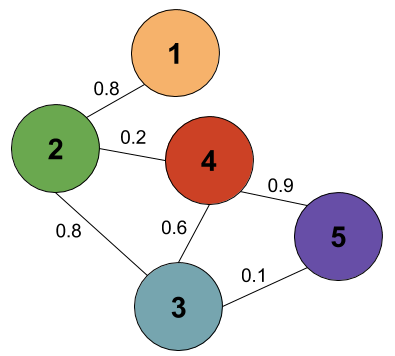
\includegraphics[width=0.8\linewidth]{./figures/multicut.png}
	\caption{An example of the benefits of using multicut over simpler agglomeration schemes. If we input this example into a na\"ive agglomeration strategy that collapses all edges with a threshold greater than 0.5, this entire segment will merge together despite the fact that nodes 2 and 4 and nodes 3 and 5 have low affinities.}
	\label{fig:multicut}
\end{figure}

Applying a top-down globally optimal partitioning function allows us to enforce some domain-specific constraints on the reconstruction.
In connectomics, we want to enforce the topological restrictions that each partition in the graph has a genus of zero. 
The greedy-additive heuristic solves the multicut graph partitioning problem by enforcing this constraint.
Previous agglomeration strategies at the per-region level consider neighboring superpixels in order of merge probability. 
These superpixels are clustered hierarchically without concern for global constraints.
We compare the benefits of a top-down partitioning function versus the traditional bottom-up clustering methods.

\subsection{Variation of Information}

We evaluate the performance of our methods using the split version of the variance of information~\cite{meila2003comparing}. 
Consider a ground truth labeling $GT$ and our automatically reconstructed segmentation $SG$. 
Over and undersegmentation are quanitified by the conditional entropy $H(GT | SG)$ and $H(SG | GT)$ respectively. 
Since we are measuring the entropy between two clusterings, better split variation of information scores are closer to the origin.